% Options for packages loaded elsewhere
\PassOptionsToPackage{unicode}{hyperref}
\PassOptionsToPackage{hyphens}{url}
%
\documentclass[
]{article}
\usepackage{amsmath,amssymb}
\usepackage{lmodern}
\usepackage{ifxetex,ifluatex}
\ifnum 0\ifxetex 1\fi\ifluatex 1\fi=0 % if pdftex
  \usepackage[T1]{fontenc}
  \usepackage[utf8]{inputenc}
  \usepackage{textcomp} % provide euro and other symbols
\else % if luatex or xetex
  \usepackage{unicode-math}
  \defaultfontfeatures{Scale=MatchLowercase}
  \defaultfontfeatures[\rmfamily]{Ligatures=TeX,Scale=1}
\fi
% Use upquote if available, for straight quotes in verbatim environments
\IfFileExists{upquote.sty}{\usepackage{upquote}}{}
\IfFileExists{microtype.sty}{% use microtype if available
  \usepackage[]{microtype}
  \UseMicrotypeSet[protrusion]{basicmath} % disable protrusion for tt fonts
}{}
\makeatletter
\@ifundefined{KOMAClassName}{% if non-KOMA class
  \IfFileExists{parskip.sty}{%
    \usepackage{parskip}
  }{% else
    \setlength{\parindent}{0pt}
    \setlength{\parskip}{6pt plus 2pt minus 1pt}}
}{% if KOMA class
  \KOMAoptions{parskip=half}}
\makeatother
\usepackage{xcolor}
\IfFileExists{xurl.sty}{\usepackage{xurl}}{} % add URL line breaks if available
\IfFileExists{bookmark.sty}{\usepackage{bookmark}}{\usepackage{hyperref}}
\hypersetup{
  pdftitle={Metabolic variation project},
  hidelinks,
  pdfcreator={LaTeX via pandoc}}
\urlstyle{same} % disable monospaced font for URLs
\usepackage[margin=1in]{geometry}
\usepackage{graphicx}
\makeatletter
\def\maxwidth{\ifdim\Gin@nat@width>\linewidth\linewidth\else\Gin@nat@width\fi}
\def\maxheight{\ifdim\Gin@nat@height>\textheight\textheight\else\Gin@nat@height\fi}
\makeatother
% Scale images if necessary, so that they will not overflow the page
% margins by default, and it is still possible to overwrite the defaults
% using explicit options in \includegraphics[width, height, ...]{}
\setkeys{Gin}{width=\maxwidth,height=\maxheight,keepaspectratio}
% Set default figure placement to htbp
\makeatletter
\def\fps@figure{htbp}
\makeatother
\setlength{\emergencystretch}{3em} % prevent overfull lines
\providecommand{\tightlist}{%
  \setlength{\itemsep}{0pt}\setlength{\parskip}{0pt}}
\setcounter{secnumdepth}{-\maxdimen} % remove section numbering
\ifluatex
  \usepackage{selnolig}  % disable illegal ligatures
\fi

\title{Metabolic variation project}
\author{}
\date{\vspace{-2.5em}}

\begin{document}
\maketitle

{
\setcounter{tocdepth}{2}
\tableofcontents
}
Cara A. Gallagher\\
Postdoctoral researcher\\
University of Potsdam\\
Notebook started: November 4th, 2021

\hypertarget{project-focus}{%
\paragraph{Project focus:}\label{project-focus}}

\hypertarget{collaborators}{%
\paragraph{Collaborators:}\label{collaborators}}

\begin{center}\rule{0.5\linewidth}{0.5pt}\end{center}

\hypertarget{entry-template}{%
\subsubsection{Entry: template}\label{entry-template}}

\hypertarget{general-information}{%
\paragraph{General information:}\label{general-information}}

\textbf{Date}:\\
\textbf{Author}: Cara A. Gallagher\\
\textbf{Trace tag}:\\
\textbf{Keyword}:\\
\textbf{Title}:\\
\textbf{Overview}:\\
\textbf{Files}:

\hypertarget{specific-details}{%
\paragraph{Specific details:}\label{specific-details}}

\begin{center}\rule{0.5\linewidth}{0.5pt}\end{center}

\hypertarget{entry-november-5th-2021}{%
\subsubsection{Entry: November 5th,
2021}\label{entry-november-5th-2021}}

\hypertarget{general-information-1}{%
\paragraph{General information:}\label{general-information-1}}

\textbf{Date}: 05/11/2021\\
\textbf{Author}: Cara A. Gallagher\\
\textbf{Trace tag}: Data evaluation\\
\textbf{Keyword}: Parameterization\\
\textbf{Title}: Estimating BMR parameters\\
\textbf{Overview}: Estimating BMR normalization constant and slope from
published data\\
\textbf{Files}:\\
*
\textasciitilde/EBIVRProject/Data/Parameterization/BMR/SadowskaEtAl2015.xlsx\\
* \textasciitilde/EBIVRProject/Scripts/Input
scripts/EBIV\_BMR\_parameter\_estimation.R

\hypertarget{specific-details-1}{%
\paragraph{Specific details:}\label{specific-details-1}}

\begin{itemize}
\tightlist
\item
  Set up files for initial parameterization of BMR parameter values\\
\item
  Data used for first run freely available from the Supplement of:

  \begin{itemize}
  \tightlist
  \item
    Sadowska, E.T., Stawski, C., Rudolf, A., Dheyongera, G., Chrząścik,
    K.M., Baliga-Klimczyk, K. and Koteja, P., 2015. Evolution of basal
    metabolic rate in bank voles from a multidirectional selection
    experiment. Proceedings of the Royal Society B: Biological Sciences,
    282(1806), p.20150025.\\
  \end{itemize}
\item
  Using the basic MTE equation format of:

  \begin{itemize}
  \tightlist
  \item
    \(M_B = B_0m^γ\)
  \end{itemize}
\item
  Used \emph{gls} function from ``nlme'' package\\
\item
  Used data from control (C) and herbivorous (H) selection lines, since
  these had similar BMR values in the paper\\
\item
  Tested a lm, glm, and three gls models, and assessed fit using AIC

  \begin{itemize}
  \tightlist
  \item
    Simple gls gave the best fit\\
  \end{itemize}
\item
  Will use mean values for now, then variation can be added later\\
\item
  Output plot:
\end{itemize}

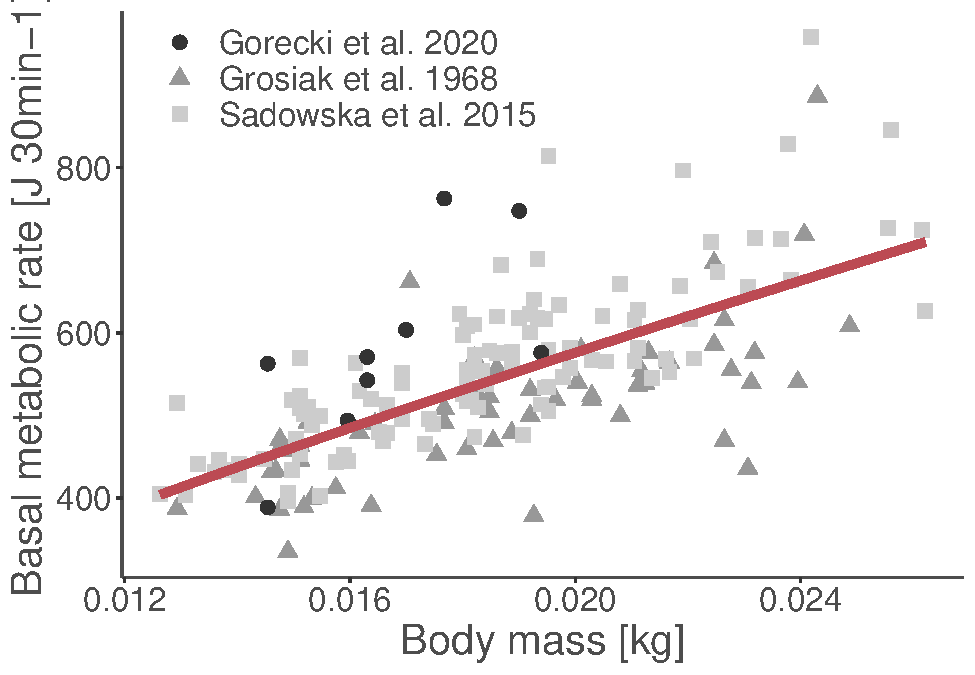
\includegraphics{EBIVnotebook_files/figure-latex/unnamed-chunk-1-1.pdf}

\begin{center}\rule{0.5\linewidth}{0.5pt}\end{center}

\hypertarget{general-information-2}{%
\paragraph{General information:}\label{general-information-2}}

\textbf{Date}: 09-11-2021\\
\textbf{Author}: Cara A. Gallagher\\
\textbf{Trace tag}: Conceptual model evaluation\\
\textbf{Keyword}: Conceptual design decisions\\
\textbf{Title}: Planning cost of transport modelling\\
\textbf{Overview}: Deciding on an approach for modelling movement costs
\textbf{Files}:\\
* \textasciitilde/EBIVRProject/Scripts/Input
scripts/EBIV\_COT\_approach\_decision.R

\hypertarget{specific-details-2}{%
\paragraph{Specific details:}\label{specific-details-2}}

\begin{itemize}
\tightlist
\item
  Basing on Pontzer 2016 - \url{https://doi.org/10.1098/rsbl.2015.0935}

  \begin{itemize}
  \tightlist
  \item
    Model for energy costs of legged locomotion, including costs of
    Activation-Relaxation and Cross-brdige cycling (ARC model)\\
  \item
    Can be used for flat ground running, incline/decline running, or
    climbing\\
  \item
    Power can be modelled to vary curvilinearly with speed, but
    ``speed-related increase in cross-bridge cost is unlikely to be
    evident in small animals, for which cross-bridge costs account for a
    very small portion of Ė and ECOT'', so I have decided to use the
    linear approximation\\
  \end{itemize}
\item
  Compared a few other published estimates in the R script, more can be
  added later\\
\item
  Decided to use Pontzer equation to estimate incremental COT (though
  lower than other equations) because it included a wide variety of
  species and gives a more updated estimate\\
\item
  Postural costs will be added separately based on the average
  percentage increase over RMR in Chappell et al.~2004, Dlugosz et
  al.~2009, and Rezende et al.~2006 (all on mice)

  \begin{itemize}
  \tightlist
  \item
    Making costs mass dependent is consistent with findings in Chappell
    et al 2013 doi.org/10.1242/jeb.079186\\
  \item
    Also costs did not change with ambient temperature in Chappell. et
    al 2004\\
  \end{itemize}
\item
  So total costs of transport will be based on iCOT (function of speed)
  + PCOT (as BMR * 2.159 (or 215.9\%))\\
\item
  With this setup seems to get a pretty similar output value to those of
  Rezende et al.~2006, for similarly sized animals\\
\item
  Example plot showing costs by speed divied up into iCOT (dark blue),
  PCOT (teal), and BMR (coral) (left) and minCOT by mass (right):
\end{itemize}

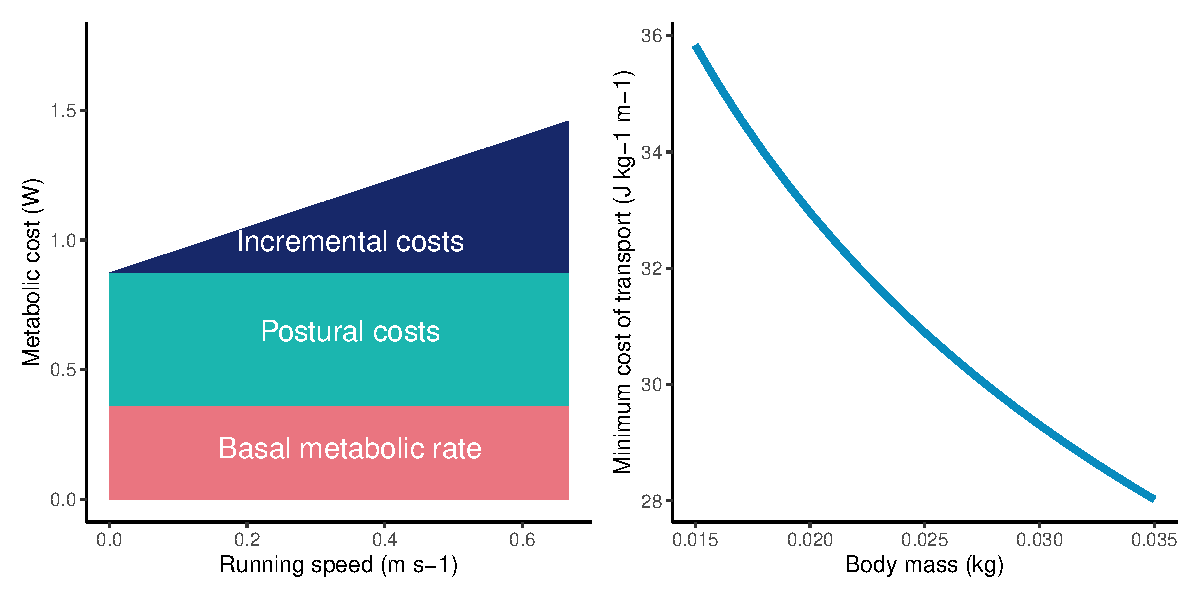
\includegraphics{EBIVnotebook_files/figure-latex/unnamed-chunk-2-1.pdf}
\includegraphics{EBIVnotebook_files/figure-latex/unnamed-chunk-2-2.pdf}
\includegraphics{EBIVnotebook_files/figure-latex/unnamed-chunk-2-3.pdf}
\includegraphics{EBIVnotebook_files/figure-latex/unnamed-chunk-2-4.pdf}

\begin{center}\rule{0.5\linewidth}{0.5pt}\end{center}

\end{document}
